\documentclass[a4paper, 14pt]{extarticle}

\usepackage[T2A]{fontenc}
\usepackage{natbib}
\usepackage{graphicx}
\usepackage[english, russian]{babel}
\usepackage{fontspec}
\usepackage{amsmath}
\usepackage{amsfonts}
\usepackage{amssymb}
\usepackage{amsthm}
\usepackage{mathtools}
\usepackage{mathrsfs}
\usepackage{icomma}
\usepackage{fullpage}
\usepackage{ulem}
\usepackage{setspace}
\usepackage{listings}
\usepackage{indentfirst}
\usepackage[left=2cm,right=1.5cm,top=2cm,bottom=2cm]{geometry}
\usepackage{xcolor}
\usepackage{float}
\usepackage{csquotes}
\usepackage{hyperref}
\usepackage{graphics}



\definecolor{urlcolor}{HTML}{0000FF} % цвет гиперссылок
\definecolor{linkcolor}{HTML}{000000} % цвет гиперссылок
\hypersetup{pdfstartview=FitH, linkcolor=linkcolor, urlcolor=urlcolor, colorlinks=true}


\setmainfont{Times New Roman}
\setlength{\parindent}{5ex}
\setlength{\parskip}{1em}
\renewcommand{\baselinestretch}{1}

\graphicspath{{images/}}


\definecolor{buzzlightyear}{HTML}{8757A5}
\definecolor{grass}{HTML}{738D06}
\definecolor{literal}{HTML}{F18A2B}
\definecolor{commentcolor}{HTML}{8E908B}

\lstdefinestyle{habrstyle}{
    backgroundcolor=\color{white},
    commentstyle=\color{commentcolor},
    keywordstyle=\bfseries\color{buzzlightyear},
    numberstyle=\tiny\color{commentcolor},
    stringstyle=\color{grass},
    basicstyle=\ttfamily\footnotesize,
    breakatwhitespace=false,
    breaklines=true,
    captionpos=b,
    keepspaces=true,
    numbers=left,
    numbersep=5pt,
    showspaces=false,
    showstringspaces=false,
    showtabs=false,
    tabsize=4
}

\lstset{style=habrstyle}

\begin{document}
    % НАЧАЛО ТИТУЛЬНОГО ЛИСТА
    \begin{center}
        \begin{center}
            \hfill \break
            \normalsize{Санкт-Петербургский государственный политехнический}\\
            \normalsize{университет Петра Великого}\\
            \hfill \break
            \normalsize{\textbf{Высшая школа интеллектуальных систем и}}\\
            \normalsize{\textbf{суперкомпьютерных технологий}}\\
            \hfill \break
            \hfill \break
            \hfill \break
            \normalsize{Лабораторная работа}\\
            \hfill \break
            \normalsize{\LARGE Шум}\\
        \end{center}
        \hfill \break
        \hfill \break
        \hfill \break
        \hfill \break
        \hfill \break
        \hfill \break
        \hfill \break
        \hfill \break
        \hfill \break
        \hfill \break
        \begin{tabbing}
            Выполнил студент гр. 3530901/80201 \`И.С. Иванов\\
            \\
            Преподаватель: \`Н.В. Богач\\
        \end{tabbing}
        \hfill \break
        \hfill \break
        \hfill \break
        \hfill \break
        \begin{center}
            Санкт-Петербург\\
            2021
        \end{center}
        \thispagestyle{empty}
    \end{center}
    % КОНЕЦ ТИТУЛЬНОГО ЛИСТА

    % ОГЛАВЛЕНИЕ
    \newpage
    \tableofcontents

    % СПИСОК ИЛЛЮСТРАЦИЙ
    \newpage
    \listoffigures

    % СПИСОК ЛИСТИНГОВ
    \newpage
    \lstlistoflistings

    \newpage


    \section{Упражнение №1: Изучение шума}
    \label{sec:1}

    Во первом упражнении необходимо скачать файлы с шумом природы, например дождь или морские волны.
    Выделить из этих сигналов спектры и установить, на какой шум похож каждый сигнал.

    Для выполнения были скачаны аудио файлы звука шторма и моря.

    Прочитаем файл.
    Выделим сегмент длинной в 1 секунду.
    Посмотрим на спектр выделенного сегмента.

    \begin{lstlisting}[language=Python, caption={Чтение файла, выделение фрагмента, вывод спектра}, label={lst:read_segment_spectr}]
        from thinkdsp import read_wave

        wave = read_wave('Sounds/127596__juskiddink__wind-in-birch-trees-a-passing-sheep.wav')

        segment = wave.segment(start=1.5, duration=1.0)

        spectrum = segment.make_spectrum()
        spectrum.plot_power()
    \end{lstlisting}

    \begin{figure}[H]
        \centering
        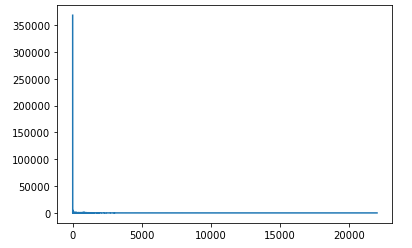
\includegraphics[width=0.8\linewidth]{wind_segment_spectr}
        \caption{Спектр сегмента}
        \label{fig:wind_segment_spectr}
    \end{figure}

    Так как большей амплитуде соответствует меньшее значение частоты, можно сказать, что это красный или розовый шум.

    Посмотрим на спектр сегмента в логарифмическом масштабе.

    \begin{figure}[H]
        \centering
        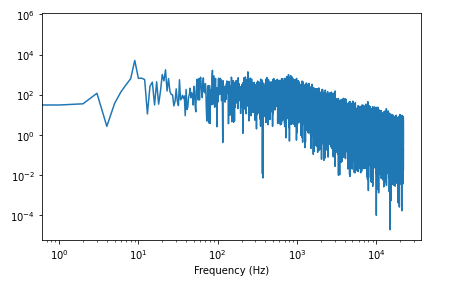
\includegraphics[width=0.8\linewidth]{wind_spectr_segment_log}
        \caption{Спектр сегмента в логарифмическом масштабе}
        \label{fig:wind_spectr_segment_log}
    \end{figure}

    Так же проверим другой сегмент сигнала.

    \begin{figure}[H]
        \centering
        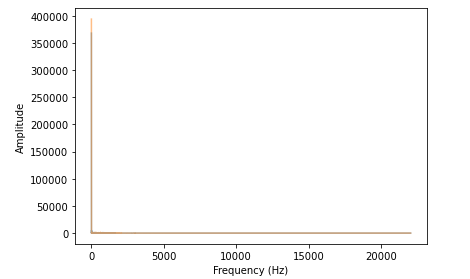
\includegraphics[width=0.8\linewidth]{wind_segment_1_and_2_spectr}
        \caption{Наложенные спектры двух сегментов}
        \label{fig:wind_segment_1_and_2_spectr}
    \end{figure}

    На основании спектра этого сегмента так же можно сказать, что это красный или розовый шум.

    \begin{figure}[H]
        \centering
        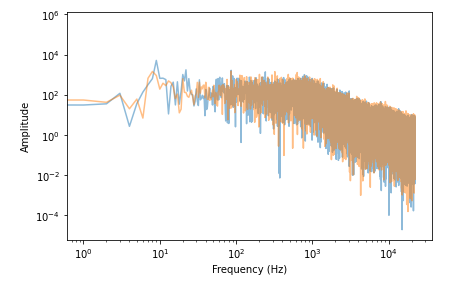
\includegraphics[width=0.8\linewidth]{wind_segment_1_and_2_spectr_log}
        \caption{Наложенные спектры двух сегментов в логарифмическом масштабе}
        \label{fig:wind_segment_1_and_2_spectr_log}
    \end{figure}

    На графике видно, что сигнал не сильно меняется с течением времени.

    \begin{figure}[H]
        \centering
        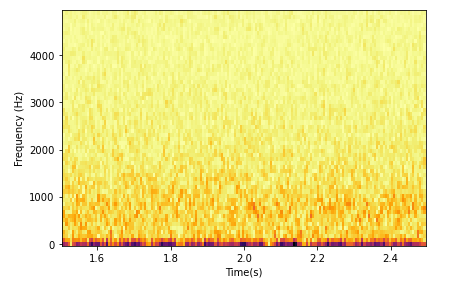
\includegraphics[width=0.8\linewidth]{wind_segment_spectrogram}
        \caption{Спектрограмма сегмента}
        \label{fig:wind_segment_spectrogram}
    \end{figure}

    Изучим файл со звуками морских волн.
    Выделим сегмент длинной в 1 секунду.
    Посмотрим на спектр выделенного сегмента.

    \begin{figure}[H]
        \centering
        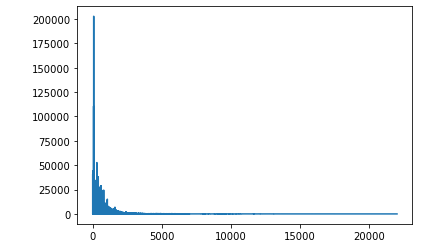
\includegraphics[width=0.8\linewidth]{sea_segment_spectr}
        \caption{Спектр сегмента}
        \label{fig:sea_segment_spectr}
    \end{figure}

    Так как большей амплитуде соответствует меньшее значение частоты, можно сказать, что это красный или розовый шум.

    Посмотрим на спектр сегмента в логарифмическом масштабе.

    \begin{figure}[H]
        \centering
        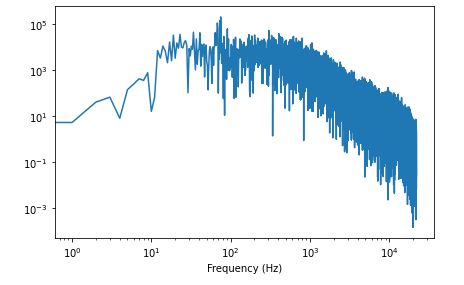
\includegraphics[width=0.8\linewidth]{sea_segment_spectr_log}
        \caption{Спектр сегмента в логарифмическом масштабе}
        \label{fig:sea_segment_spectr_log}
    \end{figure}

    Так же проверим другой сегмент сигнала.

    \begin{figure}[H]
        \centering
        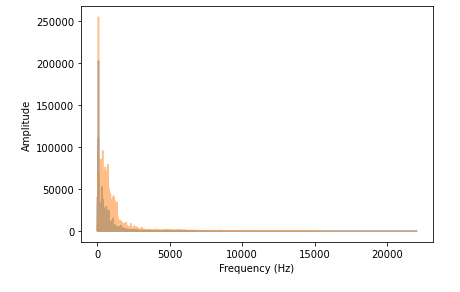
\includegraphics[width=0.8\linewidth]{sea_segment_1_and_2_spectr}
        \caption{Наложенные спектры двух сегментов}
        \label{fig:sea_segment_1_and_2_spectr}
    \end{figure}

    На основании спектра этого сегмента так же можно сказать, что это красный или розовый шум.

    \begin{figure}[H]
        \centering
        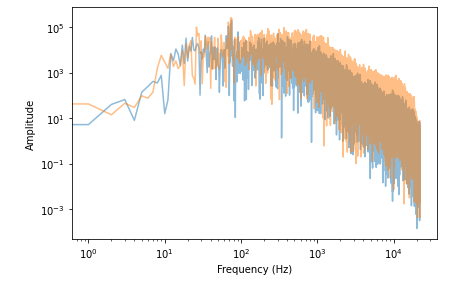
\includegraphics[width=0.8\linewidth]{sea_segment_1_and_2_spectr_log}
        \caption{Наложенные спектры двух сегментов в логарифмическом масштабе}
        \label{fig:sea_segment_1_and_2_spectr_log}
    \end{figure}

    На графике видно, что сигнал не сильно меняется с течением времени.

    \begin{figure}[H]
        \centering
        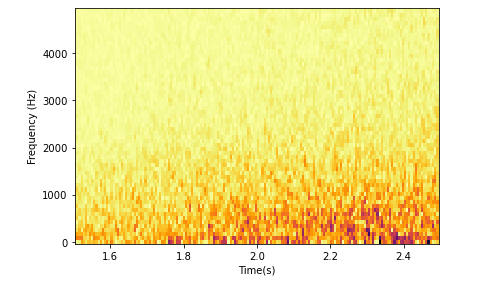
\includegraphics[width=0.8\linewidth]{sea_segment_spectrogram}
        \caption{Спектрограмма сегмента}
        \label{fig:sea_segment_spectrogram}
    \end{figure}

    \newpage


    \section{Упражнение №2: метод Бартлетта}
    \label{sec:2}

    Во втором упражнении необходимо реализовать метод Бартлетта и использовать его для оценки спектра мощности шумового сигнала.

    Реализуем метод Бартлетта:

    \begin{lstlisting}[language=Python, caption= Метод Бартлетта, label={lst:method_bartlett}]
        from thinkdsp import Spectrum

        def bartlett_method(wave, seg_length=512, win_flag=True):
            spectro = wave.make_spectrogram(seg_length, win_flag)
            spectrums = spectro.spec_map.values()
            psds = [spectrum.power for spectrum in spectrums]
            hs = np.sqrt(sum(psds) / len(psds))
            fs = next(iter(spectrums)).fs
            spectrum = Spectrum(hs, fs, wave.framerate)
            return spectrum
    \end{lstlisting}

    Проверим работу метода.
    Вызовем метод дважды для двух сегментов из предыдущего упражнения и выведем полученные спектры на график:

    Выведем конец сигнала.

    \begin{figure}[H]
        \centering
        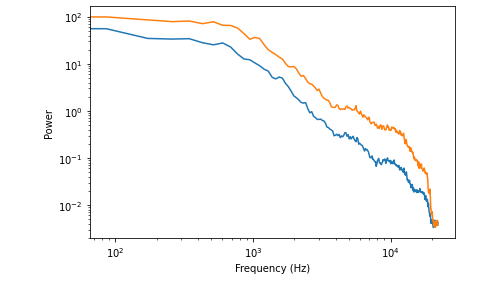
\includegraphics[width=0.8\linewidth]{sea_segment_1_and_2_Bartlett}
        \caption{Спектры после использования метода Бартлетта}
        \label{fig:sea_segment_1_and_2_Bartlett}
    \end{figure}

    Изучив полученные спектры, можно сделать вывод, что в них есть связь между частотой и амплитудой.
    Зависимость линейная.

    \newpage


    \section{Упражнение №3: Получение спектра курса валюты Bitcoin}
    \label{sec:3}

    В третьем упражнении нам необходимо скачать CSV файл c историческим данными курса Bitcoin.
    Необходимо вычислить спектр цен как функцию времени и установить, на какой шум похож спектр.

    Считаем файл:

    \begin{lstlisting}[language=Python, caption= Считывание файла, label={lst:read_bitcoin}]
        import pandas as pd

        data = pd.read_csv('Res/BTC_USD_2013-10-01_2021-05-04-CoinDesk.csv',
                           parse_dates=[0])
    \end{lstlisting}

    Посмотрим на график полученных данных:

    \begin{lstlisting}[language=Python, caption= Построение графика, label={lst:make_bitcoin_wave}]
        ys = data['Closing Price (USD)']
        ts = data.index

        from thinkdsp import Wave

        wave = Wave(ys, ts, framerate=1)
        wave.plot()
        decorate(xlabel='Time (days)')
    \end{lstlisting}

    \begin{figure}[H]
        \centering
        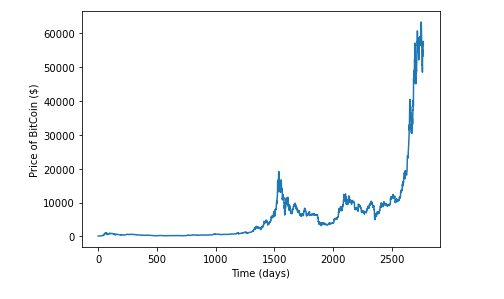
\includegraphics[width=0.8\linewidth]{bitcoin_wave}
        \caption{График курса Bitcoin}
        \label{fig:bitcoin_wave}
    \end{figure}

    Построим логарифмический спектр курса Bitcoin

    \begin{figure}[H]
        \centering
        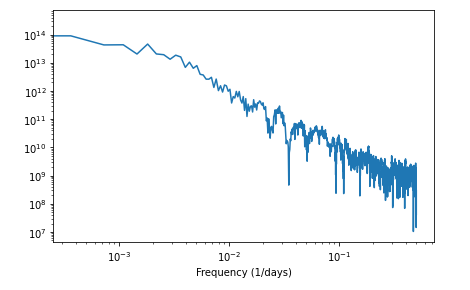
\includegraphics[width=0.8\linewidth]{bitcoin_spectrum}
        \caption{Логарифмический спектр курса Bitcoin}
        \label{fig:bitcoin_spectrum}
    \end{figure}

    Из спектра можно понять, что это розовый или красный шум.

    Посмотрим на "slope", полученного спектра.

    "Slope" равен -1.7835653687618445.

    Для красного шума характерно значение -2, значит курс Bitcoin является розовым шумом.

    \newpage


    \section{Упражнение №4: UncorrelatedPoissonNoise}
    \label{sec:4}

    В четвертом упражнении необходимо реализовать класс \texttt{UncorrelatedPoissonNoise}, наследующий \texttt{Noise} и предоставляющий \texttt{evaluate}.
    Необходимо сгенерировать случайные величины из распределения Пуассона, а так же пару секунд \texttt{UP} и прослушать.
    При малых значениях \texttt{amp} звук будет похож на счетчик Гейгера, а при больших на белый шум.
    Вычислить и вывести спектр для этих сигналов.

    Напишем класс \texttt{UncorrelatedPoissonNoise}:

    \begin{lstlisting}[language=Python, caption= Класс UncorrelatedPoissonNoise, label={lst:uncorrelated_poisson_noise}]
        from thinkdsp import Noise

        class UncorrelatedPoissonNoise(Noise):
            def evaluate(self, ts):
                ys = np.random.poisson(self.amp, len(ts))
                return ys
    \end{lstlisting}

    Создадим сигнал с \texttt{amp} = 0.001 и прослушаем.

    \begin{lstlisting}[language=Python, caption= Создание и прослушивание сигнала, label={lst:make_uncorrelated_poisson_noise_audio}]
        amp = 0.001
        framerate = 10000
        duration = 1

        signal = UncorrelatedPoissonNoise(amp=amp)
        wave = signal.make_wave(duration=duration, framerate=framerate)
        wave.make_audio()
    \end{lstlisting}

    Получившийся звук похож на счетчик Гейгера.

    Сверим ожидаемое количество частиц и полученное.

    \begin{lstlisting}[language=Python, caption= Сравнение ожидаемых частиц и полученных, label={lst:compare_result}]
        expected = amp * framerate * duration
        actual = sum(wave.ys)
        print(expected, actual)
    \end{lstlisting}

    \begin{figure}[H]
        \centering
        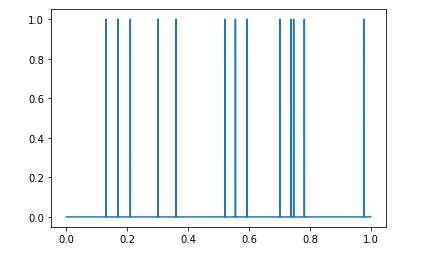
\includegraphics[width=0.8\linewidth]{poisson_wave}
        \caption{Спектрограмма полученного звука}
        \label{fig:poisson_wave}
    \end{figure}

    Посмотрим на логарифмический спектр.

    \begin{figure}[H]
        \centering
        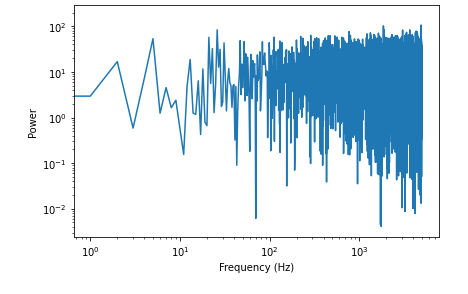
\includegraphics[width=0.8\linewidth]{poisson_log_spectrum}
        \caption{Логарифмический спектр полученного звука}
        \label{fig:poisson_log_spectrum}
    \end{figure}

    "Slope" = 0.03737836229373747.

    На основе полученных данных, можно сделать вывод, что это белый шум.

    \newpage


    \section{Упражнение №5: Алгоритм Voss-McCartney}
    \label{sec:5}

    В пятом упражнении необходимо реализовать алгоритм Voss-McCartney, вычислить спектр и убедиться, что соотношение между мощностью и частотой соответствующие.

    Реализуем алгоритм Voss-McCartney:

    \begin{lstlisting}[language=Python, caption= Алгоритм Voss-McCartney, label={lst:alg_voss_mccartney}]
        def voss(nrows, ncols=16):
            array = np.empty((nrows, ncols))
            array.fill(np.nan)
            array[0, :] = np.random.random(ncols)
            array[:, 0] = np.random.random(nrows)

            n = nrows
            cols = np.random.geometric(0.5, n)
            cols[cols >= ncols] = 0
            rows = np.random.randint(nrows, size=n)
            array[rows, cols] = np.random.random(n)

            df = pd.DataFrame(array)
            df.fillna(method='ffill', axis=0, inplace=True)
            total = df.sum(axis=1)

            return total.values
    \end{lstlisting}

    Создадим, выведем график и прослушаем сигнал, полученный с помощью этого алгоритма.

    \begin{figure}[H]
        \centering
        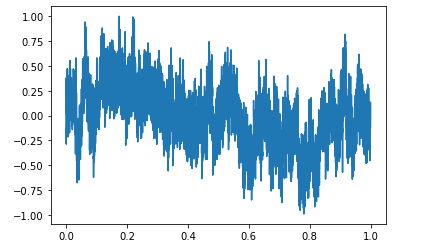
\includegraphics[width=0.8\linewidth]{voss_wave}
        \caption{График полученного сигнала}
        \label{fig:voss_wave}
    \end{figure}

    Посмотрим на логарифмический график, чтобы убедиться в правильности зависимости амплитуды от частоты.

    \begin{figure}[H]
        \centering
        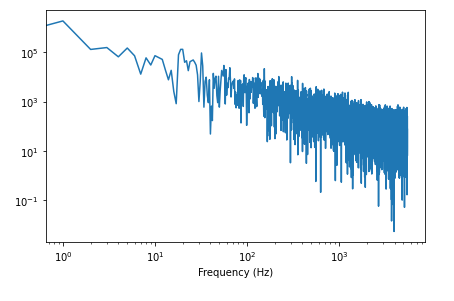
\includegraphics[width=0.8\linewidth]{voss_spectrum_log}
        \caption{Логарифмический график полученного сигнала}
        \label{fig:voss_spectrum_log}
    \end{figure}

    "Slope" = -0.9913328610110239.

    Так как "Slope" близок к -1, можно сделать вывод, что сигнал является розовым шумом.

    \newpage

    \section{Выводы}
    \label{sec:conclusions}

    В результате выполнения данной лабораторной работы мы изучили, понятие шума и как работать с ним.
    Также научились строить логарифмические спектры шумов.
    Были преобразованы данные курса валюты Bitcoin и представлены в виде источника изучения шума.
    Был создан класс для генерации случайных величин из распределения Пуассона и создан методы, реализующий алгоритм Voss-McCartney.

\end{document}